%
% Body
%

%%%%%%%%%%%%%%%%%%%%%%%%%%%%%%%%%%%%%%%%%%%%%%%%%%%%%%%%%%
%%%%%%%%%%%%%%%%%%%%%%%%%%%%%%%%%%%%%%%%%%%%%%%%%%%%%%%%%%
\section{Background}
\label{sec:numcutoffbackground}
%%%%%%%%%%%%%%%%%%%%%%%%%%%%%%%%%%%%%%%%%%%%%%%%%%%%%%%%%%
%%%%%%%%%%%%%%%%%%%%%%%%%%%%%%%%%%%%%%%%%%%%%%%%%%%%%%%%%%

%%%%%%%%%%%%%%%%%%%%%%%%%%%%%%%%%%%%%%%%%%%%%%%%%%%%%%%%%%
\subsection{The measure space and operators}
%%%%%%%%%%%%%%%%%%%%%%%%%%%%%%%%%%%%%%%%%%%%%%%%%%%%%%%%%%

We work on the probability space $(X,\mathcal{A},\mu)$. We take $S: X
\to X$ to be a transformation (or map) that is non-singular and
measurable. We choose $\mu$ to be the Borel measure. In the measure
space $(X,\mathcal{A},\mu)$ we define the following operators.
%\begin{definition} {\bfseries (Markov operator)}
%Any linear operator $M:L^1 \rightarrow L^1$ satisfying
%(a) $Mf \ge 0$ for $f\ge 0, f \in L^1$; and
%(b) $||Mf|| = ||f||$ for $f\ge 0, f \in L^1$
%is called a Markov operator.
%\end{definition}

\begin{definition}[Perron-Frobenius operator]
The Perron-Frobenius operator $P:L^1(X) \to L^1(X)$ associated with
$S$ satisfies
\begin{equation}
  \int_A (P \omega)(x)\mu(dx) = \int_{S^{-1}(A)} \omega(x)\mu(dx)
\end{equation}
for every $\omega \in L^1(X)$ and $A \in \mathcal{A}$.
\end{definition}
The Perron-Frobenius operator is linear. Because of our choice of
measure space, the Perron-Frobenius operator can be interpreted as a
map that evolves probability density functions. Also, suppose that
$\bar{\omega}$ is an invariant measure of $S$, so that
\begin{equation}
   \bar{\omega}(S^{-1}(A)) = \bar{\omega}(A)  \text{ for all } A \in \mathcal{A}.
\end{equation}
Then we have (omitting $x$)
\begin{eqnarray}
  P \bar{\omega} = \bar{\omega}.
\end{eqnarray}
%Suppose $S$ is invertible and since it is measure preserving, we have
% \begin{eqnarray}
% P_Sf(x) = f(S^{-1}(x))
% \end{eqnarray}

\todo{MW: I changed ``the invariant measure'' to ``an invariant
  measure''. It isn't generally unique?}

\todo{MW: For consistency we should always write $P(\omega)$ or $P
  \omega$. I tend to value the latter to suggest its linearity.}

\begin{definition}[Koopman operator]
Let $f \in L^\infty(X)$. The operator $U:L^{\infty}(X) \to
L^{\infty}(X)$ defined by
 \begin{eqnarray}
 Uf(x) = f(S(x))
 \end{eqnarray}
is called the Koopman operator associated with $S$.
\end{definition}
The Koopman operator is adjoint to Perron-Frobenius operator, which we
write as $U = P^*$.

\todo{MW: I added the domain to the function spaces above, so we have
  $L^\infty(X)$ rather than just $L^\infty$. Should we also add the
  range to make it completely clear? That is,
  $L^\infty(X,\mathbb{R})$?}

%%%%%%%%%%%%%%%%%%%%%%%%%%%%%%%%%%%%%%%%%%%%%%%%%%%%%%%%%%
\subsection{Notion of a cutoff}
%%%%%%%%%%%%%%%%%%%%%%%%%%%%%%%%%%%%%%%%%%%%%%%%%%%%%%%%%%

In some Markov Chains, certain probability distributions converge to
an equilibrium via a sharp transition, which becomes sharper for
larger chains. This phenomenon is referred to as \emph{cutoff} in the
finite Markov chain literature \cite{Diaconis2005, Chen2006}. Here we
extend the usual definition slightly to accommodate converge to
non-zero distance values.

\todo{MW: Why don't we compute the variance of the $f^k_n$ after
  subtracting the invariant distribution, or something, so that we
  really converge to zero?
  
  TC: We discussed this before. When the diffusion is not zero, the 
  stationary distribution is always uniform. However, Standard Map 
  has non-chaotic regions, so as the diffusion decreases, each of the 
  trajectories in Figure 2 goes to zero with decreasing exponential 
  decay rate (the second largest eigenvalue). And even in the 
  normalized plot, the decay rate is still decreasing, so for fixed 
  $k/t_n$ (say, $k/t_n=3$), we can expect $\text{var}(f_n^k)$ to 
  converge to a constant, but it is not stationary. It is the 
  eigenvector connrsponding to the second largest eigenvalue. 
  }
  

\todo{MW: I think we should name this $d$ so that we can refer to it
  below in the definition of cutoff. Does it have a standard name? If
  not, maybe we should call it a distance function?}

To any finite set $\Omega$ and any pair of probability measures
$\omega$, $\bar{\omega}$ on $\Omega$ we associate a real number
$d(\omega,\bar{\omega})$ such that
\begin{subequations}
\label{eqn:defn_d}
\begin{align}
d(\omega,\bar{\omega}) &\in [0,1] \\
d(\omega,\bar{\omega}) &= 0 \text{ if and only if } \bar{\omega}=\omega \\
\max_{\Omega,\omega,\bar{\omega}} d(\omega,\bar{\omega}) &= M_d.
\end{align}
\end{subequations}
Note that $d$ need not satisfy the triangle inequality and so is not a
metric.

\todo{MW: Should the max above really be over all $\Omega$ as well? It
  seems to be we only have one $\Omega$.}

\todo{MW: Should the max above be a sup? Why do we know the max is
  achieved?}

\todo{MW: Check that the not-a-metric comment above is correct.}

Consider a sequence of finite probability spaces $(\Omega_n)$ for $n =
1,2,\ldots$. We think of $n$ as the size of the space. Each space is
equipped with a probability measure $\bar{\omega}_n$ which we think of
as the unique invariant measure of a Markov chain on $\Omega_n$. For
each $n$ we now take a sequence of probability measures $\omega_n^k$
for $k = 0,1,2,\ldots$ such that
\begin{equation}
\lim_{k \rightarrow \infty} d(\omega_n,\bar{\omega}_n)=0.
\end{equation}
The $\omega_n^k$ should be thought of as an initial condition
$\omega_n^0$ and then iterates of the distribution under the
evolution of a Markov chain.

\todo{MW: The above paragraphs are a bit of a mess, but somehow I
  wanted to explain what the objects are. Do we want the $\omega$ to
  be pdfs, or do we rather want them to be functions on $\Omega$?}

\todo{MW: Use ldots ($\ldots$) rather than $...$ to get better
  spacing.}

The definition of a cutoff follows.
\begin{definition}[Cutoff]
\label{cutoffdefinitionn}
Take a family $(\Omega_n,\bar{\omega}_n,
(\omega^k_n)_{k=0}^{\infty})_{n=1}^{\infty}$ of finite probability
spaces $\Omega_n$ and probability measures $\bar{\omega}_n$ and
$\omega_n^k$. This family presents a $d$-cutoff if there exists a
sequence $(t_n)_{n=1}^{\infty}$ of positive reals such that, for any
$\epsilon \in (0,1)$,
\begin{subequations}
  \label{eqn:defn_cutoff}
  \begin{align}
    \label{eqn:defn_cutoff_1}
    \lim_{n \rightarrow \infty}d(\omega^{k_n}_n,\bar{\omega}_n) &= m \text{ if }
    k_n > (1+\epsilon)t_n \\
    \lim_{n \rightarrow \infty}d(\omega^{k_n}_n,\bar{\omega}_n) &= M \text{ if }
    k_n < (1-\epsilon)t_n
  \end{align}
\end{subequations}
\end{definition}

\todo{MW: Should we define the $t_n$ to be \emph{cutoff times}?}

\todo{MW: In the cutoff definition we don't say what the $k_n$
  are. This needs to be clarified.}

\todo{MW: Remind me why we need the $\epsilon$ in the cutoff
  definition? Why can't we just say $k_n > t_n$ and $k_n < t_n$?}

This definition is taken from \cite{Diaconis2005} with the change that
$m$ and $M$ are $0$ and $M_d$ in the original. The reason for this
modification will be clear when we present the results of Standard Map
simulation.

The definition of cutoff implies that the change of
$d(\omega_n^k,\bar{\omega}_n)$ from $M$ to $m$ happens ever more
rapidly as $n$ increases, but only in relation to the cutoff times
$t_n$. We can think of this as rescaling the each trajectory
$(\omega_n^k)_{k=0}^{\infty}$ in time by $t_n$ and seeing cutoff as
the limit of these rescaled trajectories to a step function.

%%%%%%%%%%%%%%%%%%%%%%%%%%%%%%%%%%%%%%%%%%%%%%%%%%%%%%%%%%
%%%%%%%%%%%%%%%%%%%%%%%%%%%%%%%%%%%%%%%%%%%%%%%%%%%%%%%%%%
\section{A model reduction view and the numerical strategy}
\label{sec:modelreduction}
%%%%%%%%%%%%%%%%%%%%%%%%%%%%%%%%%%%%%%%%%%%%%%%%%%%%%%%%%%
%%%%%%%%%%%%%%%%%%%%%%%%%%%%%%%%%%%%%%%%%%%%%%%%%%%%%%%%%%

%%%%%%%%%%%%%%%%%%%%%%%%%%%%%%%%%%%%%%%
\subsection{A model reduction view}
%%%%%%%%%%%%%%%%%%%%%%%%%%%%%%%%%%%%%%%

In this section we explain the numerical strategy to perform the simulation in detail. It is based on a model reduction view of Perron-Frobenius and Koopman operators, and the Advection-Diffusion process is done by performing a Markov Chain/linear system simulation in a finite-dimensional space. Although we make this numerical strategy extremely simple in order to go up to very fine resolution, it is still worth to explain how we make the simplification step by step.     


Firstly, in the measure space $(X,\mathcal{A},\mu)$, given an invertible map $S$, let $P_S$ and $U_S$ be the Perron-Frobenius and the Koopman
operators of a map $S$. We have the following relations:
\vspace{0.15cm}
\begin{center}
\begin{tabular}{l|ll}
\label{PUtable}
& forward in time
& backward in time
\\
\hline
probability density
& $P_S$
& $P_{S^{-1}}$
\\
scalar function
& $ U_{S^{-1}} = P_{S^{-1}}^* $
& $ U_S  = P_S^*  $
\end{tabular}
\end{center}
\vspace{0.15cm}

\todo{MW: What are $A$ and $B$ here? The language below about
  ``infinite dimensional matrices'' is not mathematically meaningful
  and should be cut. It's fine to talk about $P_S$ and $U_S$ being
  dual, so long as they really are (check this).}
  
Note the above interpretation of the operators comes from the choice of $\mu$ to be the Borel measure. One can have different interpretation if the choice is different. Moreover, since $U_S$, $U_{S^{-1}}$, $P_S$, and $P_{S^{-1}}$ are all real linear operators, one can think them as matrices, and so $U_S$ is simply the transpose of $P_S$, so do $U_{S^{-1}}$ and $P_{S^{-1}}$. We can also find the relation between $P_S$ and $U_{S^{-1}}$:  
\todo{MW: Under what conditions does (\ref{ABrelation}) actually
  hold?}
\begin{eqnarray}
  \label{ABrelation}
        U_{S^{-1}}  = [\bar{\omega}^{-1}] \circ P_S \circ [\bar{\omega}],
\end{eqnarray}
where $[\bar{\omega}]f(x) =f(x) \bar{\omega}(x)$ and $ [\bar{\omega}^{-1}]f(x) =f(x)/ \bar{\omega}(x)$ for any function $f: X \to \mathbb{R}$. This result can be derived directly from the definition of the two operators. Therefore once we have obtained any one of the four operators, it is in general easy to find the other three.

The goal of this paper is to study how a scalar function is advected by a chaotic map in the near-zero diffusion limit. From the above table, the operator one needs in this situation is $U_{S^{-1}}$. For a given scalar function $f^0: X \to \mathbb{R}$, 
\begin{eqnarray}
\label{actualiteration}
 f^{k+1} = U_{S^{-1}} f^{k}, \text{ for all }k.
\end{eqnarray}
The way we actuall perform the iteration is we approximate $U_{S^{-1}}$ by a finite-dimensional Markov transition matrix $B_n \in \mathbb{R}^{n \times n}$, and use it to iterate  $f_n^0 \mathbb{R}^n $, an approximation of the given initial function. Thus,
\begin{eqnarray}
\label{approxiteration}
 f_n^{k+1} = B_n f_n^{k}, \text{ for all }k.
\end{eqnarray}
The difference between the approximate process (\ref{approxiteration}) and the actual one (\ref{actualiteration}) is treated as the numerical diffusion, and this numerical diffusion can be reduced by increasing $n$. Thus we can have a sequence of irreducible Markov transition matrices $B_n$ (and similarly $A_n$) which converge to $U_{S^{-1}}$ (and $U_S$) when $n$ goes to infinity. Each of the $B_n \in\mathbb{R}^{n \times n}$ represents a finite-dimensional approximation of $U_{S^{-1}}$. Because we treat the error between (\ref{approxiteration}) and (\ref{actualiteration}) as the added numerical diffusion, when $n$ goes to infinity, the numerical diffusion decreases to zero. The way to find $B_n$ for a given $U_{S^{-1}}$ is through the procedure of model reduction.

Begin with $B_n$. It evolves $f_n \in
\mathbb{R}^n$. We first define a map (an observer) $g_n: f(x) \mapsto
f_n $ such that
\begin{eqnarray} 
  (f_n)_i = (g_n(f(x)))_i = \int_{a_i} f(x) \mu(dx) \mbox{, for }i = 1
  \mbox{ to } n.
\end{eqnarray}
The sample space $X$ is discretized into $n$ grids $a_1,a_2,\ldots,a_n$ and each grids represents one state in the new sample space. There are various methods to find $B_n$ such that $\lim_{n\rightarrow \infty}B_n = U_{S^{-1}}$. One example is the lattice method \cite{Pierrehumbert2000}. It approximates $U_{S^{-1}}$ by a permutation
matrix, and then adds a smoothing step to make the matrix irreducible. In fact an optimal $B_n$ can be found by the techniques
of optimal model reduction \cite{Beck2007, Froyland2001, Froyland1999}: for any $f$ and $f_n = g_n(f)$, the optimal reduced
model of $U_{S^{-1}}$ is the $B_n$ such that
\begin{eqnarray}
\label{objfunction1}
  B_n f_n = \operatorname*{argmin}_{{f'_n}} || {f'_n} -g_n(U_{S^{-1}} f) ||_{\text{diag}(\sqrt{\bar{\omega}})},
\end{eqnarray}
i.e. it minimize the iteraiton error in the weighed norm space. Suppose the grids are numbered by $a_1,a_2,\ldots, a_n$. The optimal $A_n\in \mathbb{R}^{n \times n}$ satisfying~(\ref{objfunction1}) can be calculated explicitly as
  \begin{eqnarray}
    \label{Bnij}
    (B_n)_{ij} =  \frac{\bar{\omega}(S(a_j)\cap a_i)}{\bar{\omega}(a_j)}.
  \end{eqnarray}
To evaluate ($\ref{Bnij}$) requires the calculation of $S(a_j)$,
finding the area intersection, and integrating over a non-uniform
measure $\bar{\omega}$. For most of the maps, these steps can only be
done numerically.  Similarly, the optimal $A_n$, which is the best approximation of $U_S$, has the explicit form
  \begin{eqnarray}
    \label{Anija}
    (A_n)_{ij} =  \frac{\bar{\omega}(S^{-1}(a_j)\cap a_i)}{\bar{\omega}(a_j)}.
   \end{eqnarray}
One can check that the pair $\{A_n$, $B_n\}$ satisfies
 \begin{eqnarray}
  \label{AnBnrelation}
         B_n = \text{diag}({\bar{\omega}_n}^{-1}) A_n^T \text{diag}(\bar{\omega}_n),
  \end{eqnarray}
which is a discrete version of (\ref{ABrelation}). Apparently, how good
the approximation is for a certain $n$ depends on the choice of mesh
grids. In this article, we simply use regular grids: for $X =
[0,1]\times[0,1]$, each grid has size $h=1/\sqrt{n}$ in each
dimension and area $1/n$, $A_n \in \mathbb{R}^{n \times n}$.



%The proposed numerical strategy can be easily applied to 1-D maps, where $\bar{\omega}(S^{-1}(a_j)\cap a_i)$ is calculated by linear integration with measure $\bar{\omega}$ over the overlapping region of grids $S^{-1}(a_j)$ and $a_i$. For 2-D maps, numerical integration with measure $\bar{\omega}$ needs to be applied. This is in general very expensive and cannot be done for large number of grids. To give the feeling of how the number of girds relates to the approximation results, we use the mixing channel example again.

\todo{MW: The following example seems again to be irrelevant for the
  main point of the paper. I think reviewers will be confused by
  it. We should just directly define the method that we will use to
  generate the numerical results and cut the example below, I
  think. Just to make sure I understand things here, the numerical
  method described below and used for~\ref{mixingcrosssectionreduced}
  is not the method used to generate the final numerical results,
  right?}

The proposed numerical strategy can be easily applied to 1-D maps, where $\bar{\omega}(S^{-1}(a_j)\cap a_i)$ is calculated by linear integration with measure $\bar{\omega}$ over the overlapping region of grids $S^{-1}(a_j)$ and $a_i$. In 2-D, it is already hard to decide whether $S(a_j)\cap a_i$ is non-empty, let alone to calculating the areas. Therefore further simplification needs to be done for high resolution. In fact, when the grid gets smaller, the variation of $\bar{\omega}$ over one grid also becomes smaller, and one can safely approximate $B_n$ by
 \begin{eqnarray}
    \label{Anijapprox}
    (B_n)_{ij} \approx  \frac{{\mu}(S(a_j)\cap a_i)}{\mu(a_j)}.
   \end{eqnarray}
To go up to extremely high resolution, we make the approximation
procedure even simpler: suppose $X = T^2$ and $S: T^2 \rightarrow
T^2$, and let the grid size be $h$ on both dimensions. We number the grids
by $a_1,a_2,\ldots, a_{n^2}$. Let $\mathbf{x}_i =(x_{1i},x_{2i})$ be the
center of grid $a_i$; then
 \begin{eqnarray}
 \label{finegridmethod}
 (B_n)_{ij} \approx \begin{cases}
   \frac{1}{4} &\mbox{if } S(x_{1j}\pm \frac{h}{2},x_{2j}\pm \frac{h}{2}) \in a_i, \\
   0           &\mbox{otherwise}. \\
 \end{cases}
 \end{eqnarray}
To evaluate (\ref{finegridmethod}) we need only map points on the grid corners. The approximation of $B_n$ has only $4$ non-zeros in each row. Compared with (\ref{Bnij}), this approximation is far from optimal, but when $n$ goes to infinity, clearly it still converges to $U_{S^{-1}}$. During the simulation, the matrix $B_n$ is never explicitly
formed. We need only store a size $n$ state vector during the iteration. This approximation ensures that the operation count of evolving the system is always a constant times $n$. Equation~(\ref{finegridmethod}) will serve as our main tool in section~\ref{sec:numresults}. 

We want to stress again that although the numerical strategy we use is just equation~(\ref{finegridmethod}), the above simplification procedure is still necessary for understanding the insight of it. We apply a similar numerical strategy in~\cite{topopt} for the mixing process of a microfluidic mixing channel. The flow map generated by the microfluidic mixing channel does not have a uniform invariant distribution. In fact, the physical intrepretation of the invariant distribution is the normal velocity profile on the cross-section of the channel. Hence the choice of the operators to assure the correct physical conservation is thus crucial for the accuracy of the result. Refer \cite{topopt} for more detail.   

\todo{MW: When referencing things we should put a non-breaking space
  just before the ref, so that it doesn't get put on a separate
  line. For example, use section~\ref{sec:numresults} rather than
  section \ref{sec:numresults}. In the above paragraph the final
  section number was appearing by itself on a line until I added the
  non-breaking space.}

\todo{MW: We should have a figure like~\ref{mixingcrosssectionreduced}
  but for the standard map and using the numerical method that we
  actually use for the numerical results section.}


%%%%%%%%%%%%%%%%%%%%%%%%%%%%%%%%%%%%%%%
\subsection{Additional smoothing steps}
%%%%%%%%%%%%%%%%%%%%%%%%%%%%%%%%%%%%%%%
Using the numerical strategy in the previous section, we can evolve a function or a probability
distribution by the map with some small numerical diffusion. The effect of numerical diffusion is
similar to physical diffusion in large scale, but their behaviors can be quite different in 
small scale, and these small-scale phenomenon might be important for a chaotic map to form its
stationary eigenfunction. Therefore to simulate the physical diffusion correctly, we need to
simulate the map with far higher resolution with some additional diffusion added. The additional
diffusion can be added either in spatial or in frequency domain. In spatial domain, we adopt
the method of adding a smoothing step used in \cite{Tsang2005}:
 \begin{eqnarray}
 \label{smoothingstep}
   f^{k+1}_{(p,q)} = \sum_{|r|,|s|\le 2}C_{|r|}C_{|s|}f^{k}_{(p,q)}
 \end{eqnarray}
with $C_0=1/8, C_1=1/4$, and $C_2=3/16$ and $(p,q)$ the two dimensional index of the grid. This creates a large-scale diffusion $D \approx h^2$, which is several times larger than the numerical diffusion we originally have \cite{Tsang2005}. We use a smoothing operator $M_n$ and $f^{k+1} = M_n(f^{k})$ to denote the above smoothing step. Alternatively, in frequency domain a two-dimensional FFT/IFFT with multiplication by a constant in between according to the wave numbers can be applied to simulate physical diffusion, too. This procedure is denoted by an operator $F_n$ and $f^{k+1} = F_n(f^{k})$. Note that the FFT/IFFT scheme is much more expensive when $n$ is large, because massive data transfer is required between the first dimension FFT/IFFT and the second dimension FFT/IFFT.


%%%%%%%%%%%%%%%%%%%%%%%%%%%%%%%%%%%%%%%%%%%%%%%%%%%%%%%%%%
%%%%%%%%%%%%%%%%%%%%%%%%%%%%%%%%%%%%%%%%%%%%%%%%%%%%%%%%%%
\section{Numerical results}
\label{sec:numresults}
%%%%%%%%%%%%%%%%%%%%%%%%%%%%%%%%%%%%%%%%%%%%%%%%%%%%%%%%%%
%%%%%%%%%%%%%%%%%%%%%%%%%%%%%%%%%%%%%%%%%%%%%%%%%%%%%%%%%%

%%%%%%%%%%%%%%%%%%%%%%%%%%%%%%%%%%%%%%%%%%%%%%%%%%%%%%%%%%
\subsection{Small diffusion}
%%%%%%%%%%%%%%%%%%%%%%%%%%%%%%%%%%%%%%%%%%%%%%%%%%%%%%%%%%

We study Standard Map on $T^2$:
   \begin{align}
   \label{Standardmap}
               x_1' &= x_1+x_2 +\epsilon \sin{2 \pi x_1}  (\mbox{ mod } 1), \nonumber\\
               x_2' &=  x_2 +\epsilon \sin{2 \pi x_1}     (\mbox{ mod } 1).
   \end{align}
This map is known to be chaotic, where $\epsilon$ is a parameter that can be adjusted to change the
behavior of the map. Various studies of how a point is advected by the map can be found,
for example, in \cite{Ott2002}. Here we mainly focus on how a
scalar function is evolved by the map with the presence of small diffusion. A simulation of Standard Map using $f^0=\cos(2\pi x_2)$, $f_n^0=g_n(f^0)$ and $n=500\times 500$ is shown in \ref{standardmapevolve}. Because this map is
volume preserved, its invariant measure is uniform, and hence by equation
(\ref{ABrelation}), $U_{S^{-1}}=P_S$. Thus there is no difference between evolving a scalar function and a
probability distribution. However, there are a few words about the notion of cutoff we need to say:
\begin{enumerate}
\item The quantity of interests in chaotic mixing is the variance of the function, and in the study of cutoff phenomenon, total variaion distance is the object that is discussed the most. There is no difficulty in setting the distance function $d(\omega,\bar{\omega})$ to be the $2$-norm as follows:
  \begin{eqnarray}
    d(\omega_n,\bar{\omega}_n) = \left(\sum_{i=1}^{n} \left( \frac{(\omega_n)_i}{(\bar{\omega}_n)_i}-1 \right)^2(\bar{\omega}_n)_i \right)^{1/2}.
  \end{eqnarray}
This corresponds to the study of $L_2$ cutoff in the cutoff terminology. When talking about Standard Map, due to the uniformity of the invariant distribution, the above distance is the same as the standard deviation of a function defined as $(f_n)_i = (\omega_n)_i/(\bar{\omega}_n)_i$ with mean $1$. Thus in all of our simulations, we scale the mean of the initial functions to be $1$ to fit the definition. 
\item It is clear that the maximal value of the 2-norm distance is $\infty$, so we need to set $M_d=\infty$ (instead of $M_d=1$ for total variation distance). In the original cutoff definition, $(M,m)$ always equals $(M_d,0)$, but the $f_n$ we are interested in are sinusoidal functions in the $x_1$ and $x_2$ directions, which do not maximize the distance function $d$. Hence we scale the standard deviation of $f^0$ to be $1$ in all the simulations and set $M$ to be 1.

\item Standard Map is known to have some non-chaotic region when $\epsilon$ is not zero, so the distance $d$ converges to a value $m \neq 0$.
\end{enumerate}

The above points explain why we need to slightly modify the definition of cutoff phenomenon given by Diaconis. 

Using the fine grids method (\ref{finegridmethod}), we can generate a sequence of $B_n = A_n^T$ to
approximate $U_{S^{-1}}$ by changing the number of mesh grids on $T^2$, and have $\lim_{n \rightarrow
\infty} B_n= U_{S^{-1}}$. To simulate the more physical diffusion, we define $\bar{B}_n = M_n \circ B_n$ and
$\tilde{B}_n = F_n \circ B_n$. The diffusion of $F_n$ is chosen to be equal to one smoothing step ($D= 1/n= h^2$) for comparison.

\begin{figure}
    \centerline{
      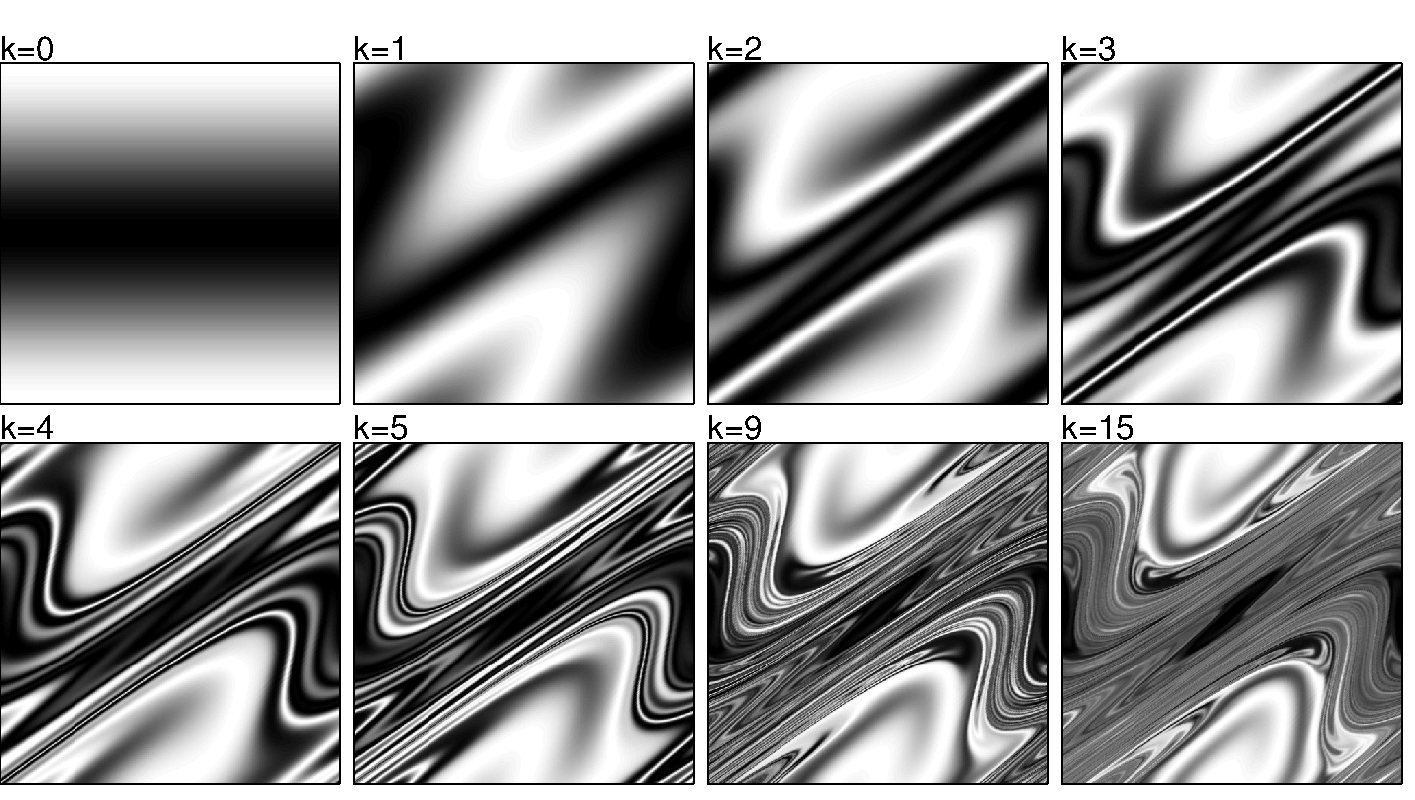
\includegraphics[width=0.8\textwidth]{standardmapevolve}
    }
    \caption{\label{standardmapevolve}For Standard Map, $\epsilon = 0.3$, $B_n$ with $n=500^2$ is applied to simulate the system with initial condition $f^0=\cos(2\pi x_2)$. The first eight iterations are plotted.}
\end{figure}




For $\epsilon = 0.3$, $n=40000^2$, $f^0=\cos(2\pi x_2)$, $f_n^0 = g_n(f^0)$. We simulate
$f_n^{k+1} =B_n f_n^k$ for $k=1$ to $20$. Each $f_n^k$ is then applied a 2-D Fourier transform to
obtain the frequency domain $\hat{f}^k_n$. The magnitude versus wave number plot is shown in the left
of Figure~\ref{freqcompare}. From this plot one can clearly observe how the chaotic map maps low
frequency components to high frequency ones (it also does the converse). Since the number of grids
is $4 \times 10^4$ by $4 \times 10^4$, the largest wave number it can catch is around $2 \times
10^4$ and it has large numerical diffusion. A major portion of components are being pushed
to high wave numbers in just a few iterations, and where diffusion works well to smooth out the corner. Once the effect of pushing and smoothing is balanced, an eigenfunction is thus formed.

To compare the difference between operators $B_n$, $\bar{B}_n$, and $\tilde{B}_n$, we do the same
simulation for all three operators. The result is plotted in the right of Figure~
\ref{freqcompare} for $k = 3,7$, and $20$. The three trajectories agree well in the low frequency part
because all kinds of diffusion have a tiny effect in low frequency terms. They begin to have
discrepancy at around wave number $2 \times 10^3$. The smoothing operator $M_n$ actually has larger
diffusion than the FFT/IFFT operator $F_n$.

The above results also explain why it is hard to simulate the function evolved by a chaotic map
correctly: very fine grids are needed to capture the high frequency terms generated in just a
few iterations.

\begin{figure}

    \centerline{
      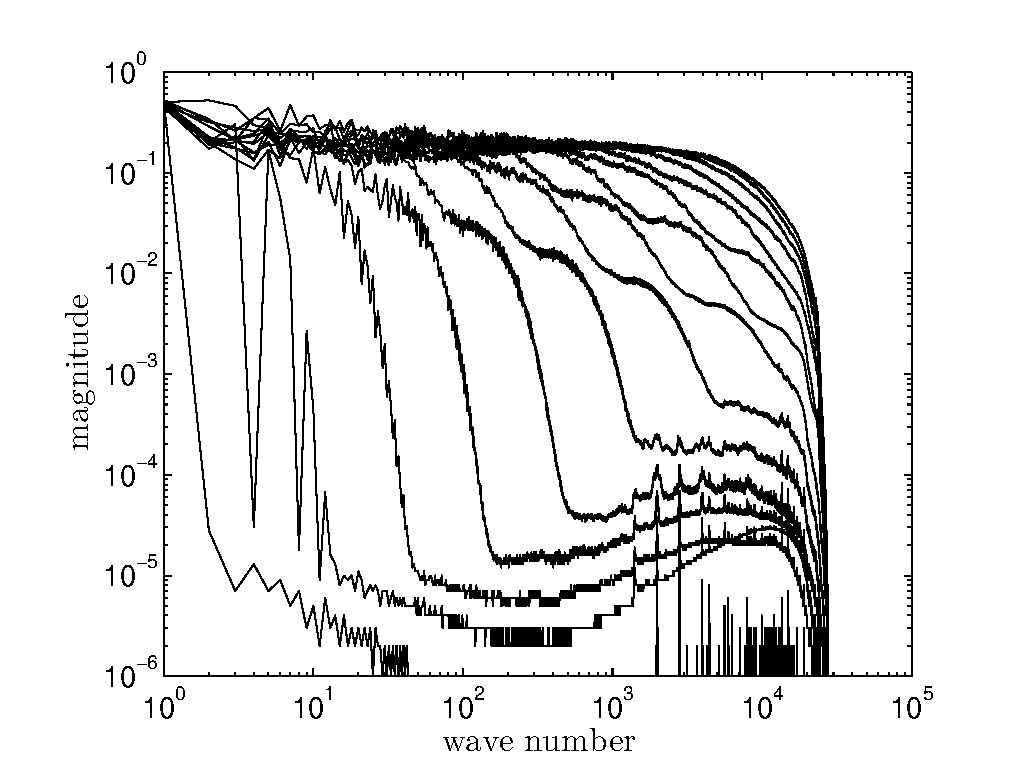
\includegraphics[width=0.5\textwidth]{standardmapfreqevolve}
      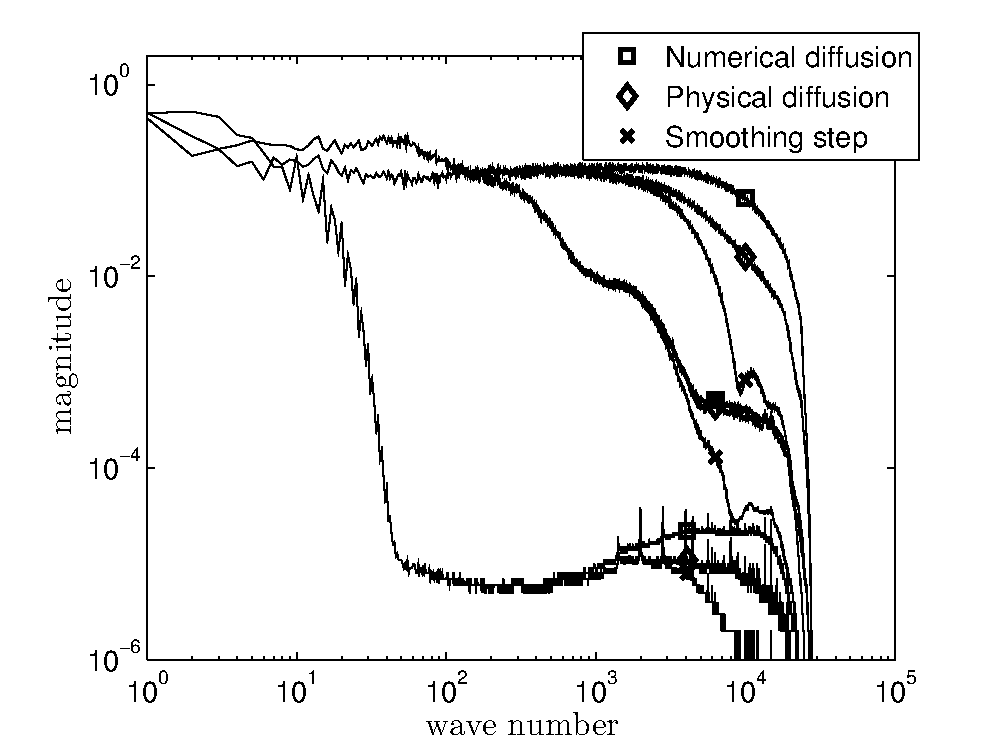
\includegraphics[width=0.5\textwidth]{standardmapfreqcompare}
    }
    \caption{\label{freqcompare}For Standard Map, $\epsilon = 0.3$, $B_n$ with $n=40000^2$ is applied to simulate the system with initial condition $f^0=\cos(2\pi x_2)$. The magnitude versus wave number plot for the first $20$ iterations is shown in the left plot. In the right plot, $B_n$, $\bar{B}_n$, and $\tilde{B}_n$ are applied to simulate the same system and the magnitude versus wave number curves are plotted for iteration $3$, $7$, and $20$.  }
\end{figure}

All three operators $B_n$, $\bar{B}_n$, and $\tilde{B}_n$ satisfying
\begin{eqnarray*}
  \lim_{n \rightarrow \infty} B_n= U_{S^{-1}}, \mbox{  }  \lim_{n \rightarrow \infty} \bar{B}_n= U_{S^{-1}}, \mbox{  }  \lim_{n \rightarrow \infty} \tilde{B}_n=U_{S^{-1}}
 \end{eqnarray*}
can be applied to study the behavior of near-zero diffusion limit of Standard Map. We choose
$B_n$ and $\bar{B}_n$ for the following studies because the computation of FFT/IFFT diffusion of $\tilde{B}_n$ is too expensive when $n$ is very large. Since their relation in the magnitude of diffusion is $B_n<\tilde{B}_n<\bar{B}_n$, if we can show both $B_n$ and $\bar{B}_n$ have similar behaviors, it is reasonable to believe that $\tilde{B}_n$ has, too.

%%%%%%%%%%%%%%%%%%%%%%%%%%%%%%%%%%%%%%%%%%%%%%%%%%%%%%%%%%
\subsection{Cutoff phenomenon}
%%%%%%%%%%%%%%%%%%%%%%%%%%%%%%%%%%%%%%%%%%%%%%%%%%%%%%%%%%


We present the main results of this article in this section. For $n$ from $2500^2$ to $80000^2$, the variance of $f^k_n$ versus iteration plots using $B_n$ and $\bar{B}_n$ as
the Koopman operators are shown in the left of Figures~\ref{standardmapun} and~\ref{smoothingstandardmapun}. The tendency is clear: when $n$ gets larger, the variances stay high ($M_B=M_{\bar{B}}=1$)
for more iterations and then drop rapidly to $m_{B} = 0.4521$ and $m_{\bar{B}}=0.4498$, respectively---they do not drop to zero because there
are unmixed ``islands''. The slope of the rapid dropping also becomes slightly milder when $n$ increases. To
justify whether they satisfy the definition of cutoff given in section~\ref{sec:numcutoffbackground}, we let $t_n$ equal the
point where each trajectory passes through $(M_{\star}+m_{\star})/2$, where $\star=\{B,\bar{B}\}$ and we normalize all trajectories by rescaling
$t_n$ to $1$. The results are plotted in the right of Figure~\ref{standardmapun} and~\ref{smoothingstandardmapun}. Although the normalized trajectories are very similar, one can still
see that when $n$ gets larger, the trajectory becomes sharper. In the left of Figure~\ref{cutofftimeandarea} we plot $t_n$ versus $1/n$ in log scale and see two straight lines. Note that for both cases, we have $D\sim O(1/n)$. Hence this plot shows that the cutoff time is inversely proportional to $\log(D)$. To see how fast the trajectories converge to their limits, we define the interpolating functions for the trajectories in the normalized plots of Figures~\ref{standardmapun} and~\ref{smoothingstandardmapun} to be $\beta_{B_n}(x)$ and $\beta_{\bar{B}_n}(x)$, where $x$ represents the normalized iteration. The function they should converge to when $n\to \infty$ is
\begin{eqnarray}
   \label{limittraj}
   \nu_{\star_\infty}(x) = \begin{cases}
                     M_{\star} &\text{ if } x<1, \\
                     m_{\star} &\text{ otherwise}, \\
                     \end{cases} 
\end{eqnarray}
where $\star=\{B,\bar{B}\}$. Define the distance between $\nu_{\star_n}(x)$ and $\nu_{\star_\infty}(x)$ to be
\begin{eqnarray}
    \label{trajdistance}
    \Delta_{\star}^l= \int_0^l | \nu_{{\star}_\infty}(x)-\nu_{{\star}_n}(x)|dx
\end{eqnarray}
for $\star=\{B,\bar{B}\}$. We calculate $\Delta^3_B$ and $\Delta^3_{\bar{B}}$ for all $\nu_{B_n}(x)$ and $\nu_{\bar{B}_n}(x)$, and plot them versus $t_n$ in the right of Figure~\ref{cutofftimeandarea}. This figure shows that when $t_n$ increases, $\Delta_{\star}^3$ decays slightly slower than linear, but clearly when $n \rightarrow \infty$, $\Delta^3_{B}$ and $\Delta^3_{\bar{B}}$ are both going down, which strongly suggests that both sequences of Markov Chains present cutoffs. 

%$\{B_n, g_n(\cos(2\pi x_2)) \}$ and $\{\bar{B}_n, g_n(\cos(2\pi x_2)) \}$ present cutoffs.

\begin{figure}
    \centerline{
      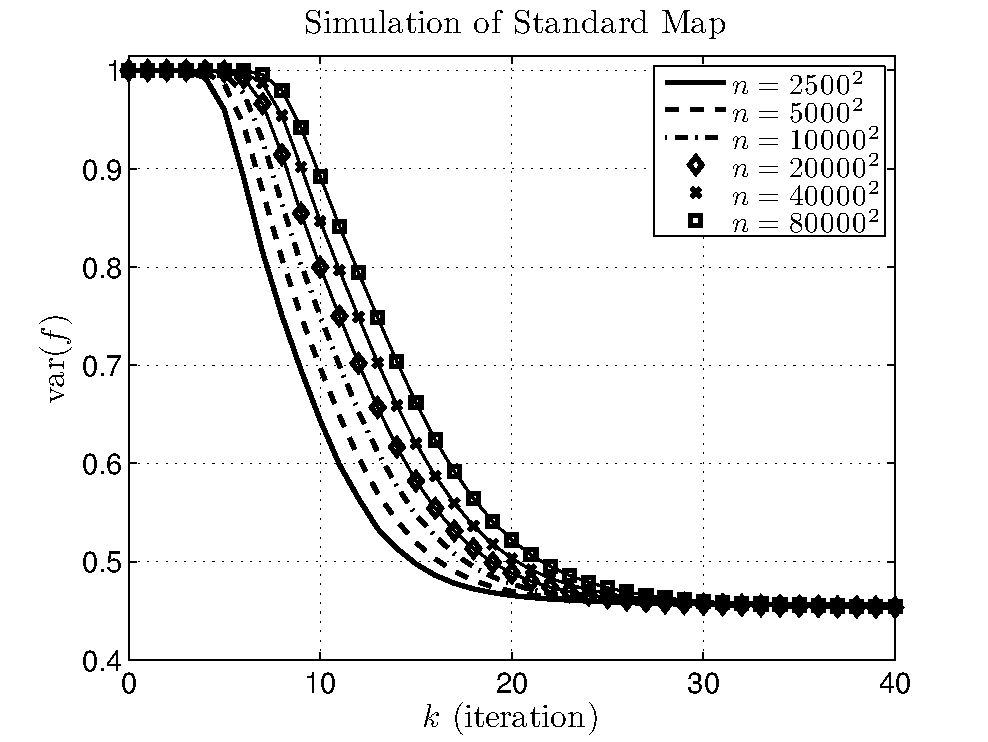
\includegraphics[width=0.5\textwidth]{standardmapcutoff}
      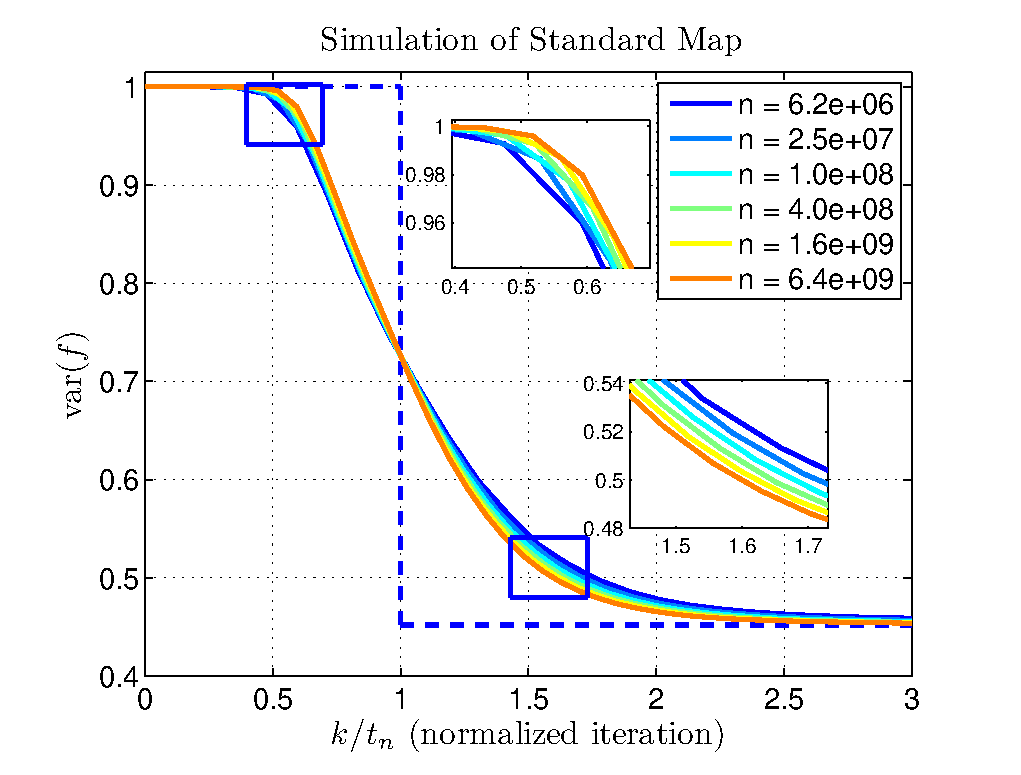
\includegraphics[width=0.5\textwidth]{standardmapcutoffn}
    }
    \caption{The left figure shows the variance of $f_n^k$ versus iteration trajectories of Standard Map simulation. We use $\epsilon=0.3$, $f^0=\cos(2 \pi x_2)$, and number of grids varies from $2500^2$ to $80000^2$. The normalized plot is shown on the right. We rescale the iteration axis and make all trajectories pass through the point $(1,0.7260)$ to observe the cutoff. The two small plots show the detailed view of the corners when trajectories have sharp change.}
 \label{standardmapun}
\end{figure}


\begin{figure}
    \centerline{
      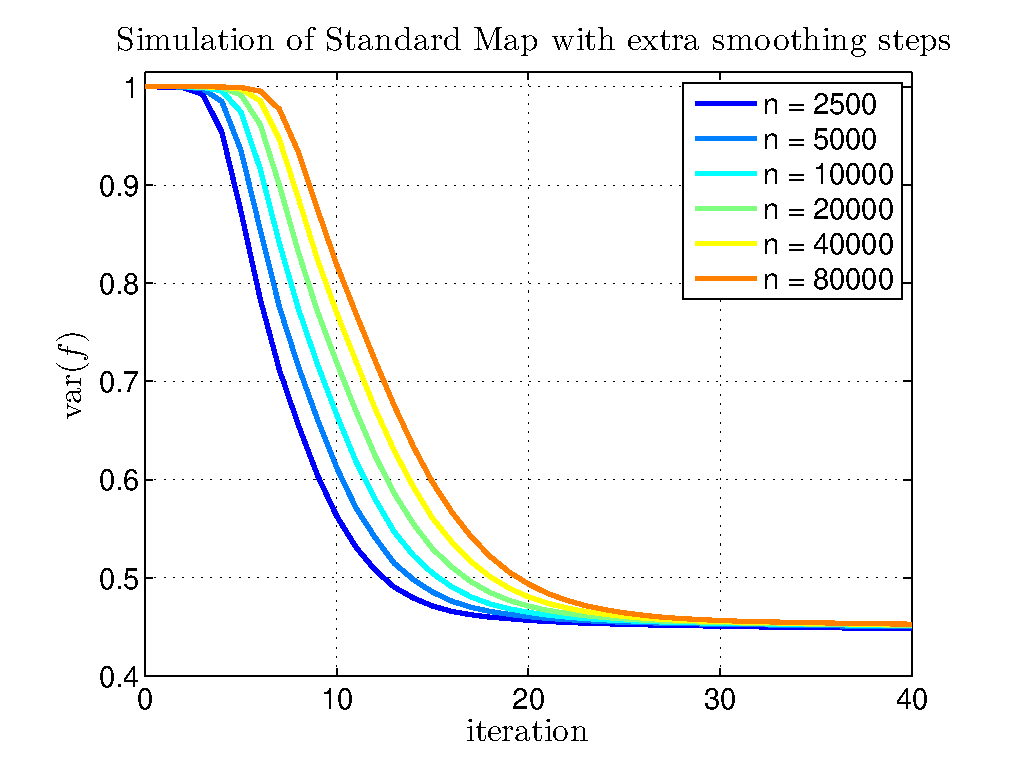
\includegraphics[width=0.5\textwidth]{standardmapcutoffwithsmoothing}
      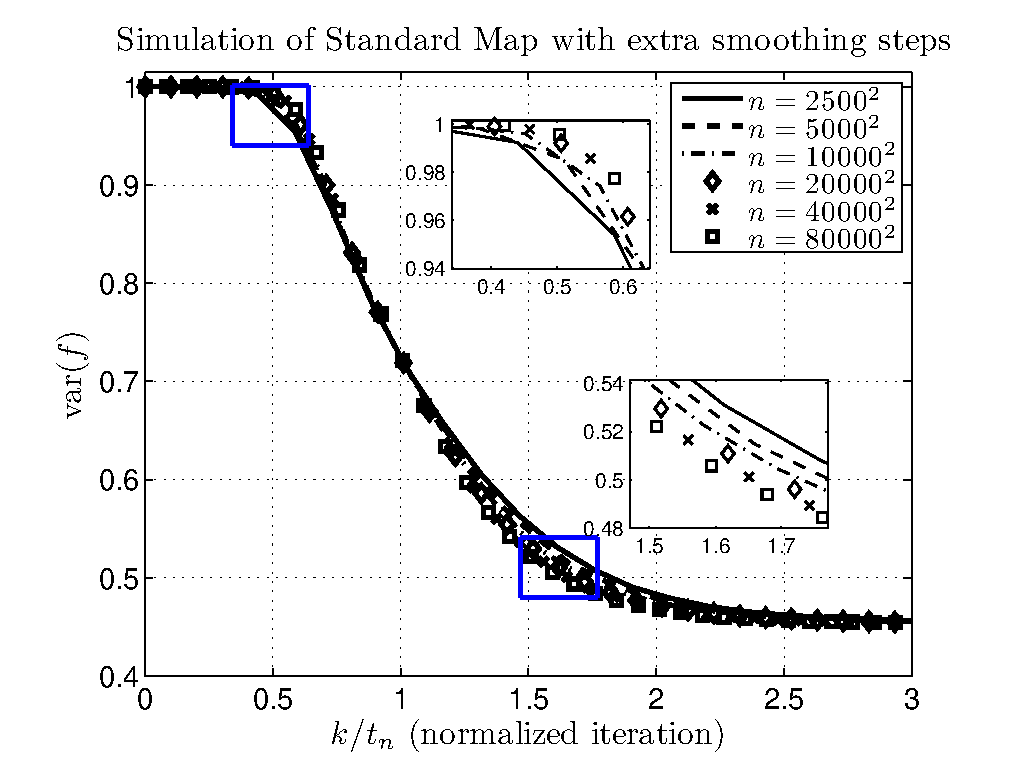
\includegraphics[width=0.5\textwidth]{standardmapcutoffwithsmoothingn}
    }
     \caption{The left figure shows the variance of $f_n^k$ versus iteration trajectories of Standard Map simulation when a smoothing step is added after each iteration. We use $\epsilon=0.3$, $f^0=\cos(2 \pi x_2)$, and the number of grids varies from $2500^2$ to $80000^2$. The normalized plot is shown in the right. We rescale the iteration axis and make all trajectories pass through the point $(1,0.7249)$ to observe the cutoff. The two small plots show the detailed view of the corners when trajectories have sharp change.}
\label{smoothingstandardmapun}
\end{figure}


\begin{figure}
   \label{cutofftime}
    \centerline{
      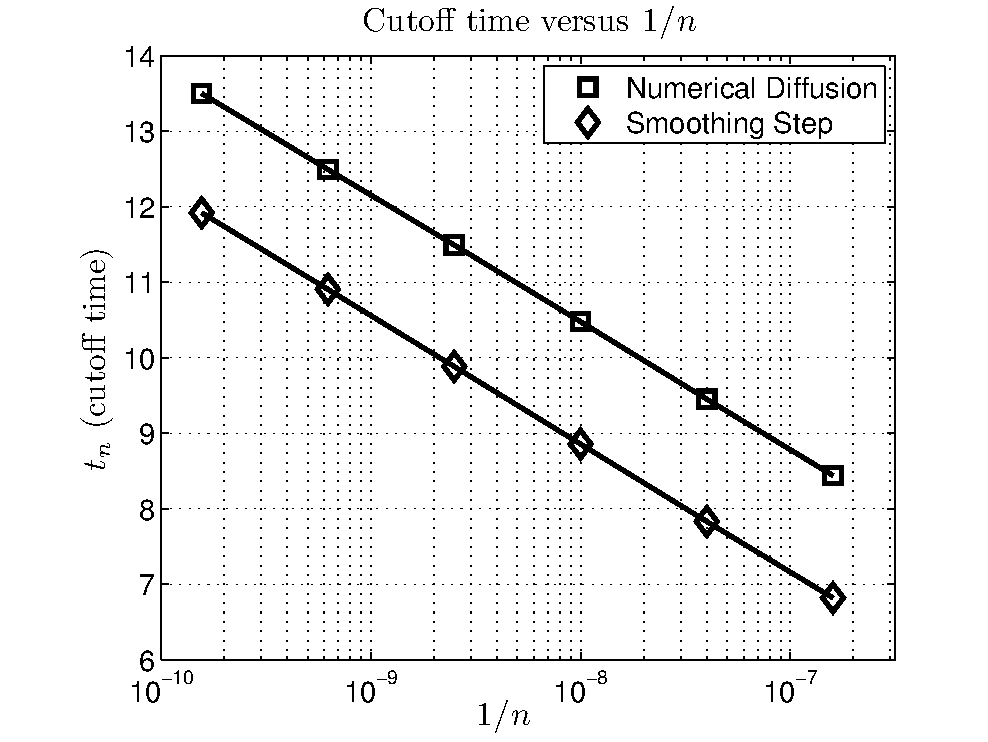
\includegraphics[width=0.5\textwidth]{cutofftimevsD}
      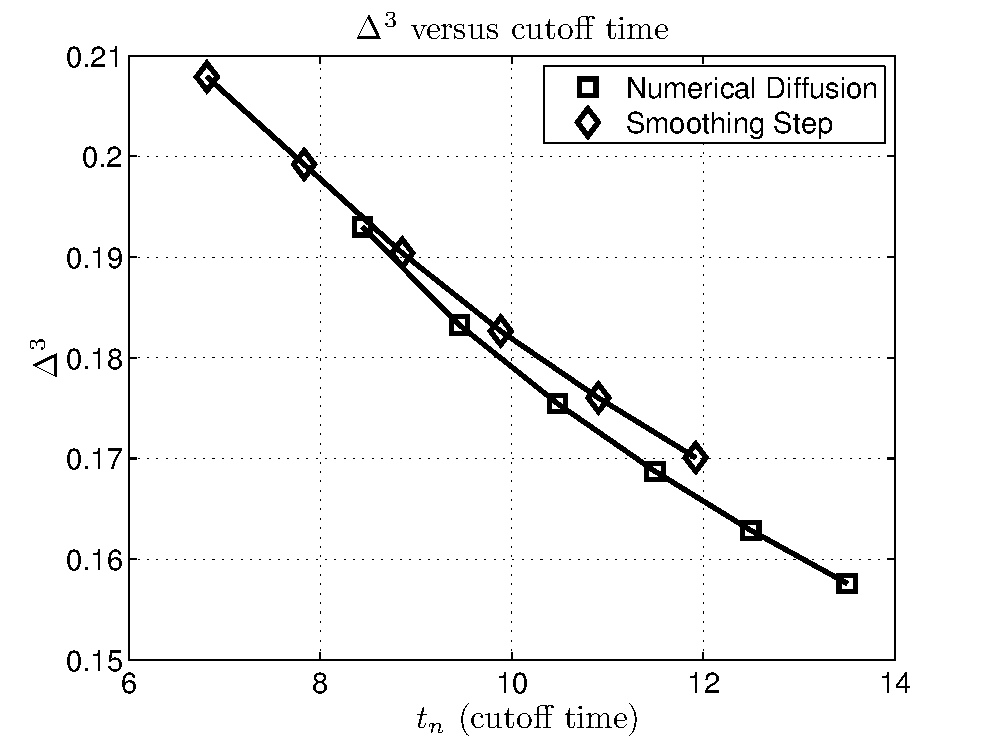
\includegraphics[width=0.5\textwidth]{areavscutofftime}
          }
     \caption{\label{cutofftimeandarea} The left plot shows how cutoff time $t_n$ relates to $1/n$ in log scale. Since we have $D \sim O(1/n) $ for our simulation strategy, one can conclude that $t_n$ is inversely proportional to $\log(D)$. The right plot shows how the normalized trajectories converge to their limit. $\Delta^3$ is defined in equation (\ref{trajdistance}). Both curves predict that when $t_n$ is very large, $\Delta^3$ goes down, and the normalized trajectory would probably become a step function.}
\end{figure}
%%%%%%%%%%%%%%%%%%%%%%%%%%%%%%%%%%%%%%%%%%%%%%%%%%%%%%%%%%
\subsection{Chaotic parameter $\epsilon$}
%%%%%%%%%%%%%%%%%%%%%%%%%%%%%%%%%%%%%%%%%%%%%%%%%%%%%%%%%%
We also study how the parameter $\epsilon$ affects the mixing trajectory when the diffusion is small. We use $f^0=\cos(2\pi x_1)$ and $f^0=\cos(2\pi x_2)$ as the initial functions and vary $\epsilon$ from $0.1$ to $0.9$. The simulation is done by $n=40000^2$ with operator $B_n$. The results are shown in Figure~\ref{standardmapparamxy}. For both initial functions and $\epsilon \ge 0.3$, the trajectories all have similar tendency. As for $\epsilon=0.1$, the trajectories show no sign of dropping in the first 50 iterations. Hence in Figure~\ref{standardmapparamsmall} we simulate $\epsilon=0$ and $0.1$ for both initial functions for $800$ iterations. One can see that for $f^0= \cos(2 \pi x_2), \epsilon=0$, the trajectory still stay almost $1$ for the first $800$ iterations, and in the case $\epsilon=0.1$ it has a small drop but we have no evidence to say it presents a cutoff or not. A more interesting thing is observed when $f^0= \cos(2 \pi x_1)$. In this case, the trajectory of $\epsilon=0$ crosses over the one of $\epsilon=0.1$ at around iteration $627$. The phenomenon that the $\epsilon=0$ map mixes faster than some other trajectories with higher $\epsilon$ is also observed in \cite{Mezic2005}. Clearly this is because when $\epsilon=0$, there is no unmixed region (no ``islands'') and so the decreasing rate of variance would not slow down by forming the eigenfunction. Hence when $\epsilon = 0$ the mixing rate only depends on whether the map is good in mixing the initial functions.

\begin{figure}
    \centerline{
      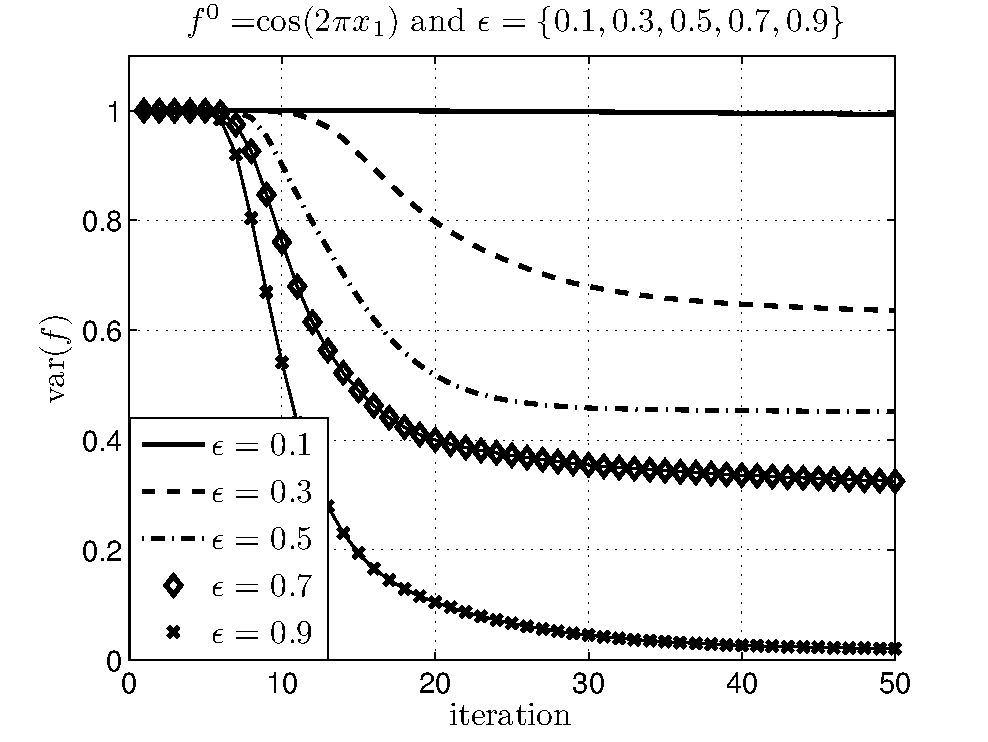
\includegraphics[width=0.5\textwidth]{standardmapparamx}
      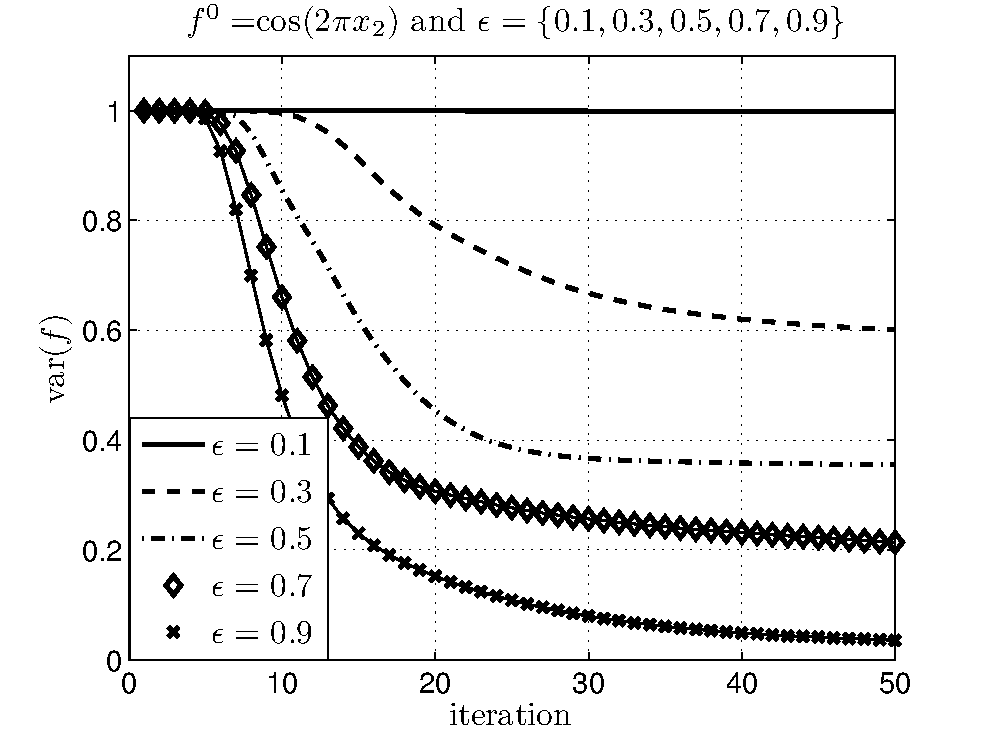
\includegraphics[width=0.5\textwidth]{standardmapparamy}
    }
    \caption{\label{standardmapparamxy} The two figures show the Standard Map simulations using $B_n$, $n=40000^2$ with different $\epsilon$ and initial function $f^0$. For $\epsilon=\{0.3,0.5,0.7,0.9 \}$ and $f^0=\{\cos{(2\pi x_1)},\cos{(2\pi x_2)}\}$, the variance trajectories all have sharp changes.}

\end{figure}


\begin{figure}
    \centerline{
      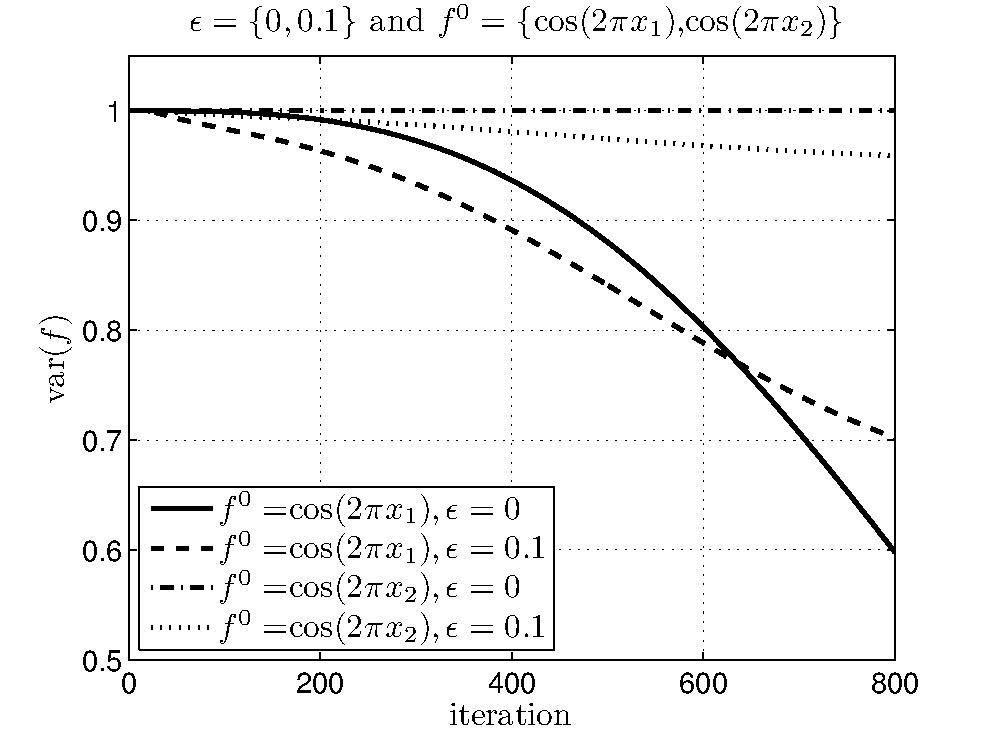
\includegraphics[width=0.5\textwidth]{standardmapparamsmall}
    }
    \caption{\label{standardmapparamsmall} This figure shows the Standard Map simulation with $\epsilon=\{0,0.1\}$ and $f^0=\{\cos{(2\pi x_1)},\cos{(2\pi x_2)}\}$. For $f^0=\cos(2\pi x_2)$, the limiting behavior of $\epsilon \rightarrow 0$ is quite clear. However, for $f^0=\cos(2\pi x_1)$, the $\epsilon=0$ trajectory crosses over the $\epsilon=0.1$ one near iteration $627$.}

\end{figure}

All the numerical results are generated by a 72-node cluster with gigabit ethernet connection. Each CPU is equipped with 1GB RAM, and the largest simulation ($80000\times80000$ number of grids) needs $51.2$GB of memory to store a state vector.



%%%%%%%%%%%%%%%%%%%%%%%%%%%%%%%%%%%%%%%%%%%%%%%%%%%%%%%%%%
\subsection{Zero diffusion and norm issues}
%%%%%%%%%%%%%%%%%%%%%%%%%%%%%%%%%%%%%%%%%%%%%%%%%%%%%%%%%%
In all above simulations we observe how the variance of a scalar function is evolved by Standard Map with small diffusion. As we have mentioned, this is equivalent to the study of $L_2$ cutoff. One may also be interested in how other norms are evolved. In the left plot of Figure~\ref{normcompare} we simulate Standard Map, $\epsilon=0.3$ and $f^0= \cos(2\pi x_1)$ by $B_n$ with $n=500^2$ and measure the following norms: $L_1$, $L_2$, $H_{-0.5}$, $H_{-1}$, and mix-norm \cite{Mezic2005}. All norms are normalized to equal $1$ at iteration $0$. Comparing with previous simulations, this one is done by very coarse grids, so one would not expect to see a very clear cutoff tendency. Nonetheless, these norms do form two groups of different behaviors: for $L_1$ and $L_2$ norms, one observes concave curves in the first few iterations, and for other norms, they drop immediately to around $0.5$ and then oscillate. 


To explain what causes this, let us consider the zero diffusion case: Standard Map is volume preserved, so without diffusion, the $L_1$ norm of the scalar function should stay constant when the function is evolved by the Koopman operator of Standard Map. Also, $L_2$ norm is invariant in the spatial and frequency domain. It is clear that the $L_2$ norm would also stay constant if there is no diffusion. For $H_{-0.5}$, $H_{-1}$, and mix-norm, they have a simple representation in frequency domain. Just the way diffusion works, to evaluate these norms, one multiplies each wave number term by a constant weight, and the weight is decreasing when the wave number increases. For 2-D domain, we plot the weights for each wave number in the right plot of Figure~\ref{normcompare} for all the norms. The diffusion weights when $D=0.01$ is also plotted on the same figure for comparison. One can conclude that the way $H_{-0.5}$, $H_{-1}$, and mix-norm work in frequency domain is very similar to diffusing the function according to a large diffusion and then evaluating their $L_2$ norms: the diffusion is very large ($D \sim 0.01$) and far from entering the region where we can observe cutoffs.  
One important feature of all $2$-D chaotic maps is the frequency cascade: it generates high wave number terms in just a few iterations, as we have seen in Figure~\ref{freqcompare}. The three norms $H_{-0.5}$, $H_{-1}$, and mix-norm suppress these terms by multiplying by small weights. The interesting cutoff phenomenon happens when diffusion is very small: $t_n\sim O(-\log(D))$. Thus these three norms lack the ability to capture things happening in small scales.

Finally we want to stress that there is no one norm that is better than another. They simply give us different information about the mixing process. The concave trajectories of $L_1$ and $L_2$ norms tell us the ``irreversibility'' feature of the chaotic system: beyond a certain iteration, it is not possible to recover the system's original state. The fast dropping trajectories of other norms show the increasing complexity of the function evolved by the chaotic map in the first few iterations.  



\begin{figure}
    \centerline{
      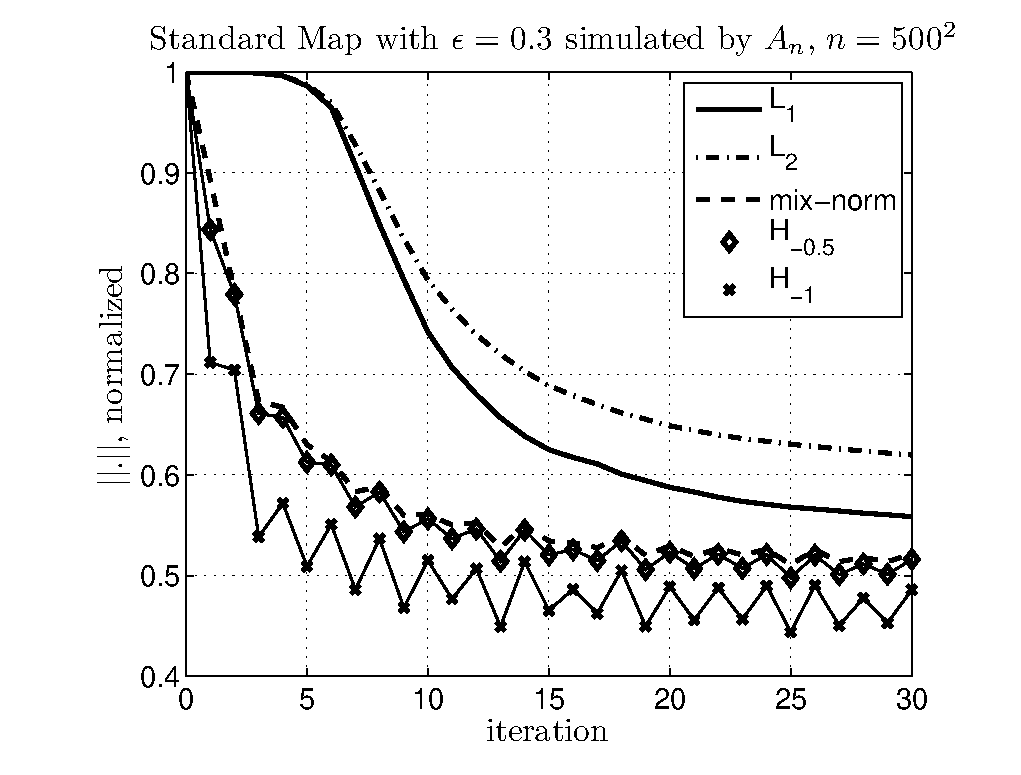
\includegraphics[width=0.5\textwidth]{normcompareplot}
      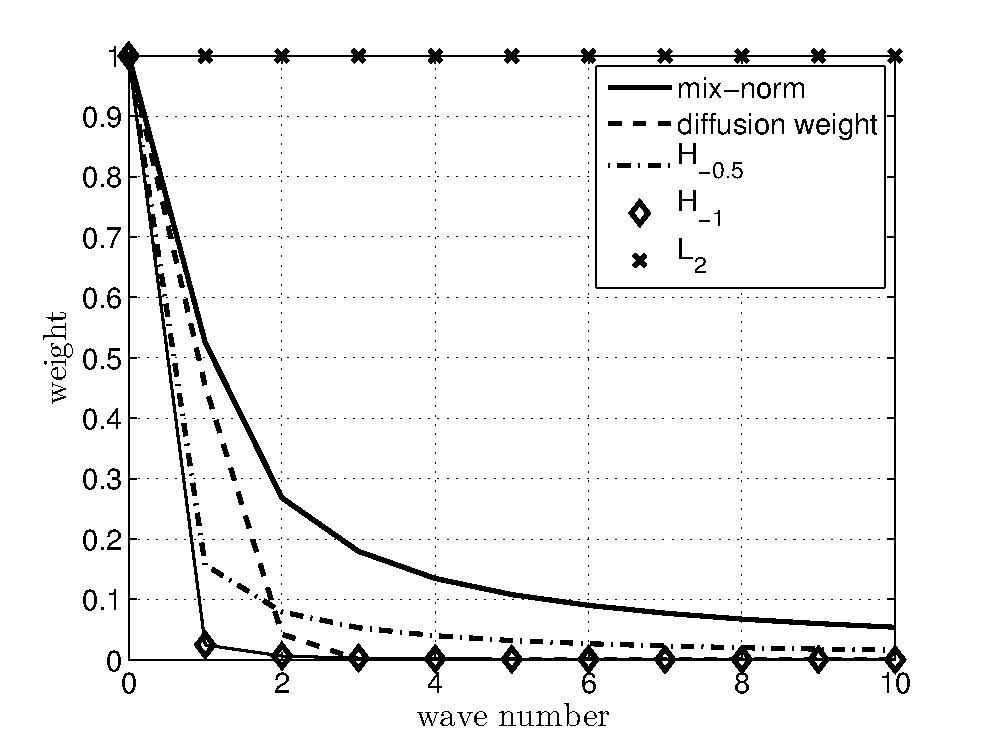
\includegraphics[width=0.5\textwidth]{normcompareweighting}
    }
    \caption{\label{normcompare} The left figure shows the Standard Map simulation with $\epsilon=0.3$ and $f^0= \cos(2\pi x_1)$. We use $B_n$ with $n=500^2$ and measure the following norms: $L_1$, $L_2$, $H_{-0.5}$, $H_{-1}$, and mix-norm. The norm trajectories form two groups: $L_1$ and $L_2$ norms show the tendency of presenting cutoffs, and the other three norms do not. In the right figure we plot the weights of $L_2$, $H_{-0.5}$, $H_{-1}$, and mix-norm at each wave number in the frequency domain. $L_2$ norm has a constant weight $1$ for all wave numbers. The other three norms have much smaller weights in large wave numbers. We also plot the diffusion weights when $D=0.01$ for comparison. One can see why these norms fail to measure the small-scale phenomena that cause cutoffs.}

\end{figure}



